\section{Технический проект}
\subsection{Общая характеристика организации решения задачи}

Необходимо спроектировать и разработать корпоративный портал учета рабочего времени сотрудников. Разрабатываемая программная система предназначена для предоставления комплексного инструмента управления временем, который позволит сотрудникам и менеджерам эффективно отслеживать и управлять временем, затраченным на проекты и задачи.

Основной принцип работы системы заключается в управлении проектами и задачами, а также в учете рабочего времени с помощью таймшитов.

Ключевым компонентом программной системы является база данных для хранения информации о пользователях, проектах, задачах и таймшитах. База данных будет обеспечивать надежное хранение данных и быстрый доступ к ним для выполнения всех операций.

Целью разработки данной программной системы является создание эффективного инструмента управления временем в корпоративной среде, который поможет повысить продуктивность сотрудников и оптимизировать процессы проектного управления, способствуя развитию и росту компании.

\subsection{Проектирование архитектуры программной системы}
\subsubsection{Выбор архитектурного стиля и паттернов проектирования}

Для разработки корпоративного портала учета рабочего времени, написанного с использованием MVC, необходимо выбрать архитектурный стиль, который обеспечит высокую производительность, безопасность и легкость поддержки.

Главным архитектурным стилем для данного проекта является Model-View-Controller (MVC). Этот архитектурный стиль разделяет приложение на три основные компонента: модель, представление и контроллер. Такая организация кода помогает четко разграничить обязанности между различными частями приложения, что делает его более модульным и легким для сопровождения.

Модель представляет данные и бизнес-логику приложения. Она включает в себя классы сущностей и контекст данных, такие как DbContext в Entity Framework. Модель отвечает за управление данными, их валидацию и выполнение бизнес-правил. Важно, чтобы модель была хорошо спроектирована, так как она служит основой для остальных компонентов приложения.

Представление отвечает за отображение данных пользователю. Представления обычно реализуются с использованием синтаксиса Razor и предназначены для представления данных в удобном и понятном формате. Они получают данные от контроллеров и отображают их на веб-странице, предоставляя пользователю интерфейс для взаимодействия с приложением.

Контроллер обрабатывает пользовательский ввод, взаимодействует с моделью и выбирает представление для отображения. Контроллеры играют ключевую роль в обработке HTTP-запросов, управлении потоками данных между моделью и представлением и обеспечении логики работы приложения.

Использование MVC архитектуры позволяет легко интегрировать другие важные компоненты, такие как безопасность через HTTPS. HTTPS (HyperText Transfer Protocol Secure) - это расширение протокола HTTP, которое обеспечивает защиту данных при их передаче через интернет с помощью SSL/TLS шифрования. Внедрение HTTPS необходимо для защиты данных пользователей и предотвращения перехвата конфиденциальной информации, такой как учетные данные сотрудников и данные о рабочем времени.

Использование архитектурного стиля MVC в сочетании с мощными возможностями платформы и SQL Server позволяет создать масштабируемое, безопасное и легко поддерживаемое приложение. Такой подход обеспечивает четкое разделение логики приложения, улучшает структурирование кода и способствует лучшей организации процесса разработки и сопровождения корпоративного портала учета рабочего времени.

Архитектура всей системы представлена на рисунке 3.1

\begin{figure}[H]
	\centering
	\includegraphics[width=0.9\linewidth]{"images/Архитектура программы"}
	\caption{Архитектура программной системы}
	\label{fig:-}
\end{figure}

\subsubsection{Структура базы данных}

Для хранения данных в корпоративном портале учета рабочего времени используется SQL Server, реляционная система управления базами данных, разработанная Microsoft. В вашем случае используется локальная установка SQL Server, что дает несколько важных преимуществ и возможностей для настройки и оптимизации.

SQL Server обеспечивает надежное и производительное решение для хранения и управления данными, необходимыми для функционирования приложения. В локальной установке вы можете полностью контролировать настройки и конфигурацию базы данных. Это включает создание и управление таблицами, представлениями, хранимыми процедурами и триггерами. Вы также можете настроить параметры производительности, безопасности и хранения в соответствии с потребностями вашего приложения.

Простое взаимодействие с базой данных через запросы из кода позволяет быстро и эффективно работать с данными. Важно оптимизировать такие запросы, чтобы обеспечить высокую производительность приложения. Использование индексов на часто используемых столбцах помогает ускорить выполнение запросов за счет быстрого доступа к нужным данным.

Одним из используемых вами механизмов являются транзакции. Транзакции обеспечивают атомарность, согласованность, изолированность и долговечность (ACID) операций с данными. Это гарантирует, что все изменения данных будут завершены успешно или не будут применены вовсе, что помогает поддерживать целостность данных. Использование транзакций особенно важно при выполнении нескольких связанных операций, которые должны быть выполнены как единое целое.

Каскадное удаление является еще одной важной функцией, используемой в вашей базе данных. Оно позволяет автоматически удалять связанные записи при удалении основной записи, что помогает поддерживать целостность данных и уменьшает риск появления "осиротевших" записей в базе данных.

Конфиденциальность и безопасность данных также играют ключевую роль. Использование файла secret.json позволяет безопасно хранить чувствительные данные, такие как строки подключения к базе данных и другие конфиденциальные настройки. Этот файл не включается в систему контроля версий, что предотвращает случайное раскрытие конфиденциальной информации.

Таким образом, использование локального SQL Server с простым взаимодействием через запросы из кода, транзакциями, каскадным удалением и файлом secret.json обеспечивает надежную, производительную и безопасную работу корпоративного портала учета рабочего времени. Эти подходы позволяют эффективно управлять данными и поддерживать высокую производительность и надежность системы.

\subsubsection{Язык программирования C\#}

C\# — это объектно-ориентированный язык программирования, разработанный компанией Microsoft. Он был создан в рамках платформы .NET и впервые представлен в 2000 году. C\# предназначен для создания разнообразных приложений, включая веб-приложения, настольные программы, игры и мобильные приложения.

\paragraph{Достоинства языка C\#}

Cовременные возможности: C\# поддерживает современные парадигмы программирования, такие как асинхронное программирование, LINQ (Language Integrated Query), и многопоточность.

Интеграция с .NET: Плотная интеграция с платформой .NET предоставляет доступ к огромной библиотеке классов и инструментов, что упрощает разработку и ускоряет процесс создания приложений.

Сильная типизация: Это снижает вероятность ошибок, связанных с типами данных, и делает код более надежным и предсказуемым.

Безопасность памяти: C\# имеет встроенные механизмы управления памятью и сборки мусора, что помогает избежать утечек памяти и других проблем, связанных с управлением памятью.

Большое сообщество и поддержка: C\# имеет обширное сообщество разработчиков и отличную документацию, что упрощает поиск решений и обмен знаниями.

\paragraph{Недостатки языка C\#}

Платформозависимость: Хотя C\# и .NET стали кроссплатформенными с выходом .NET Core, первоначально они были тесно связаны с экосистемой Windows. Некоторые старые библиотеки и инструменты могут оставаться доступными только для Windows.

Производительность: Хотя C\# и .NET оптимизированы для хорошей производительности, в некоторых случаях языки, такие как C++ или Rust, могут предложить лучшую производительность для специфичных задач, требующих максимальной эффективности.

Зависимость от среды исполнения: Приложения на C\# требуют наличия установленной среды выполнения .NET на машине пользователя, что может создавать дополнительные сложности в развертывании приложений.

\subsubsection{Библиотека ASP.net}

ASP.NET — это фреймворк для веб-программирования, разработанный компанией Microsoft, который позволяет создавать динамические веб-приложения и сервисы. Он работает на платформе .NET и поддерживает несколько языков программирования, таких как C\#, VB.NET и другие. Основные компоненты ASP.NET включают в себя веб-формы, MVC (Model-View-Controller) и веб-API.

Веб-формы (Web Forms) предоставляют удобный способ разработки веб-приложений, используя знакомую модель разработки форм, похожую на Windows Forms. Эта модель основана на событиях и компонентах, что облегчает перенос знаний и навыков разработчиков десктопных приложений в веб-среду.

ASP.NET MVC (Model-View-Controller) предлагает более гибкий и контролируемый подход к созданию веб-приложений, разделяя их на три основных компонента: модель (model), представление (view) и контроллер (controller). Это позволяет лучше организовать код, сделать его более тестируемым и поддерживаемым.

ASP.NET Web API используется для создания HTTP-сервисов, которые могут обслуживать широкий спектр клиентов, включая браузеры, мобильные устройства и традиционные десктопные приложения. Web API подходит для разработки RESTful-сервисов, что делает его отличным выбором для создания микросервисной архитектуры.

ASP.NET также предлагает мощную инфраструктуру для безопасности, включая аутентификацию и авторизацию пользователей, защиту от межсайтовых скриптов (XSS), SQL-инъекций и других распространённых угроз. Средства для обработки данных включают Entity Framework, который предоставляет удобный способ работы с базами данных на основе объектно-ориентированной модели.

\subsection{Тестирование серверной части программы}
\subsubsection{Инструмент тестирования Postman}
Postman — это популярный инструмент для тестирования и разработки API, который широко используется для отправки HTTP-запросов к серверу и анализа ответов. В частности, он удобен для тестирования URI-запросов с бекэнда и анализа JSON-файлов, которые приходят в ответах. Postman позволяет отправлять различные типы запросов, такие как GET, POST, PUT, DELETE и другие, а также настраивать параметры запросов, заголовки и тело запросов. Он предоставляет возможность легко видеть, как сервер реагирует на эти запросы, и позволяет анализировать структуру и содержимое ответов в формате JSON. Этот инструмент помогает быстро выявлять ошибки и проблемы в работе API, а также проверять корректность и соответствие ответов ожиданиям. Интуитивно понятный интерфейс Postman делает его незаменимым для разработчиков и тестировщиков, которые занимаются проверкой и отладкой серверных запросов.

\subsubsection{Результаты тестирования}

Для тестирования серверной части программы была добавлена учетная запись пользователя с логином и паролем: Admin 0000. 

Данный URI запрос отслеживает передаваемый логин и пароль. В случае нахождения пользователя в базе данных, вернется его id. Резульат тестирования логирования представлен на рисунке 3.2

\begin{figure}[H]
	\centering
	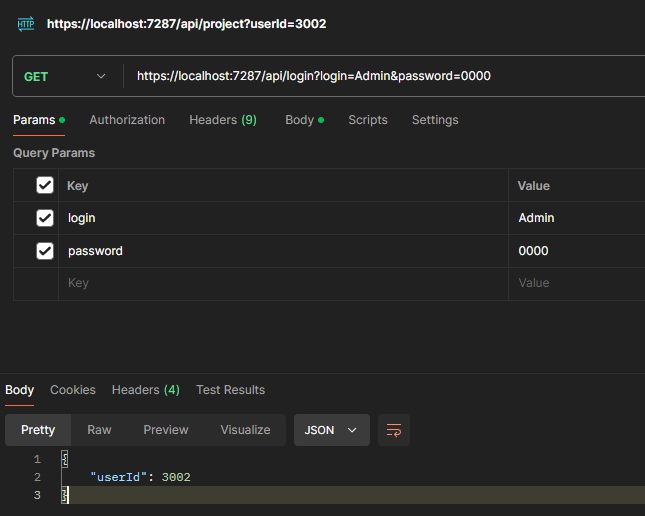
\includegraphics[width=0.7\linewidth]{images/TestURILogin}
	\caption{Возврат id пользователя по его логину и паролю}
	\label{fig:testurilogin}
\end{figure}

Данный URI запрос отслеживает передаваемый id пользователя. В случае нахождения пользователя по id, вернется его имя и фамилия. Резульат тестирования логирования представлен на рисунке 3.3

\begin{figure}[H]
	\centering
	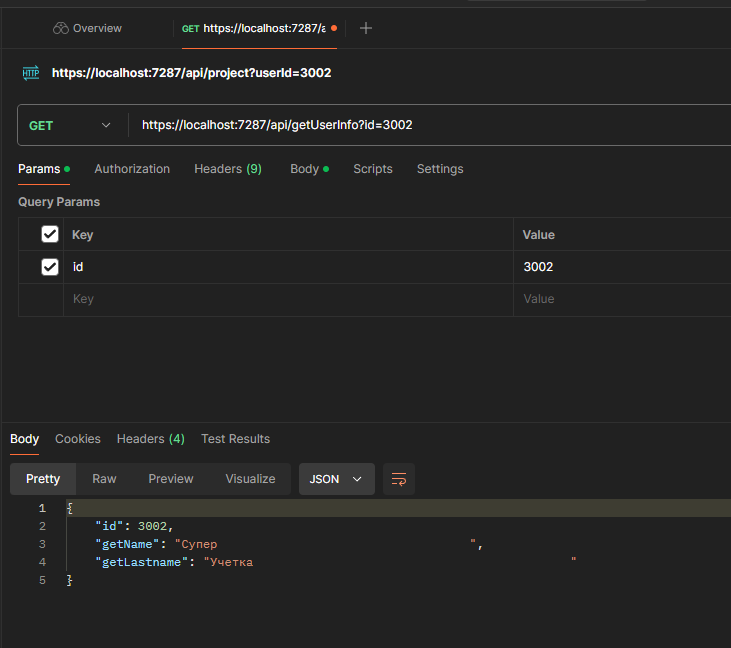
\includegraphics[width=0.7\linewidth]{images/LoginNameLastname}
	\caption{Получение имени и фамилии}
	\label{fig:loginnamelastname}
\end{figure}

На рисунке 3.4 представлен процесс получения информации по проектам пользователя по его id

\begin{figure}[H]
	\centering
	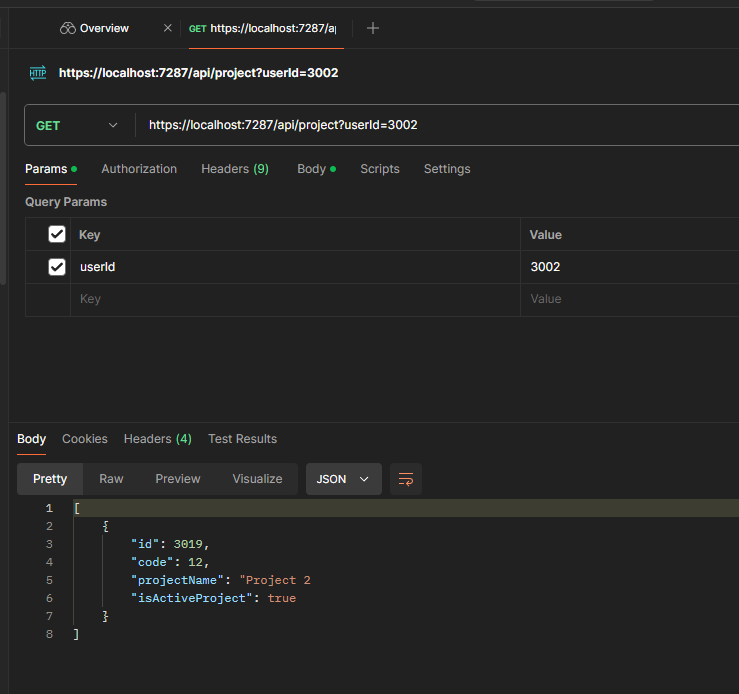
\includegraphics[width=0.6\linewidth]{images/TestGetProject}
	\caption{Получение информации по проектам}
	\label{fig:testgetproject}
\end{figure}

На рисунке 3.5 представлен процесс добаления проекта по id пользователя

\begin{figure}[H]
	\centering
	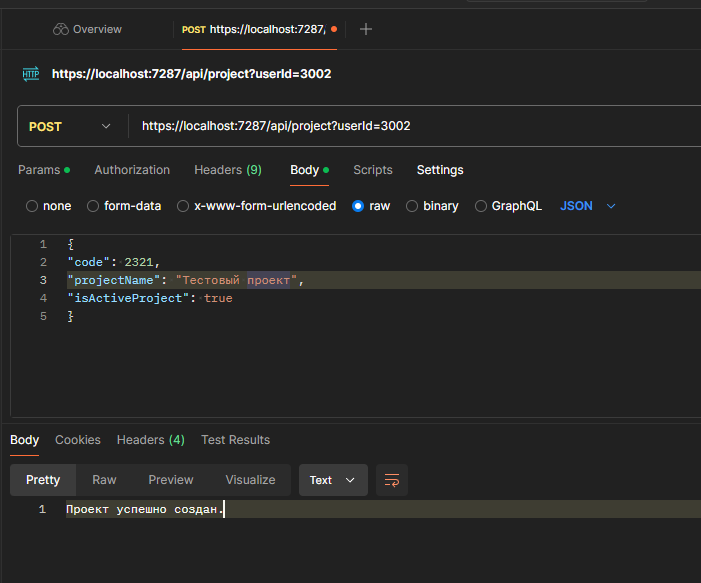
\includegraphics[width=0.65\linewidth]{images/PostProject}
	\caption{Добавление нового проекта}
	\label{fig:postproject}
\end{figure}

На рисунке 3.6 представлен процесс удаления проекта по его коду

\begin{figure}[H]
	\centering
	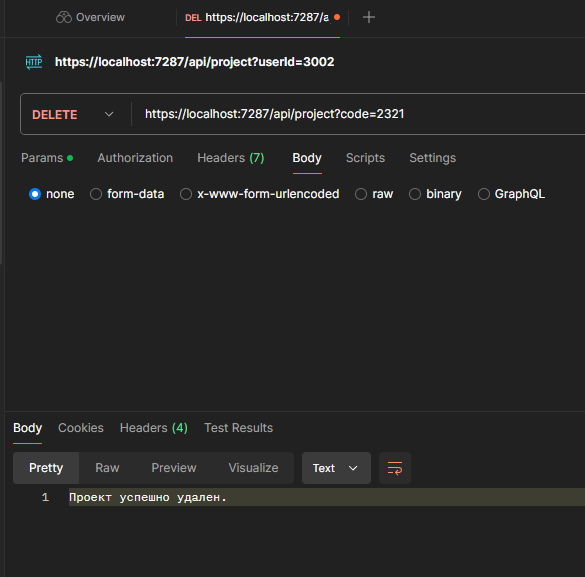
\includegraphics[width=0.7\linewidth]{images/deleteProject}
	\caption{Удаление проекта}
	\label{fig:deleteproject}
\end{figure}

На рисунке 3.7 представлен процесс изменения проекта по его коду
\begin{figure}[H]
	\centering
	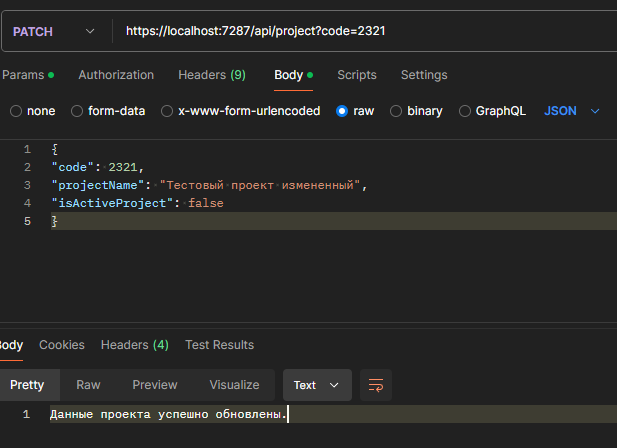
\includegraphics[width=0.7\linewidth]{images/PatchProject}
	\caption{Изменение существующего проекта}
	\label{fig:patchproject}
\end{figure}
